
\section{Sprint 1 - Summary}

In sprint 1, the main focus was planning and research, how the team is organized, requirements and test specifications. This sprint has mostly been centered around providing the right documentation to HSN, starting the project web page, as well as preparing the first oral presentation. The team had to establish a clear understanding of how to work in parallel to accomplish the build and integration of the quadcopters. 
\newline \newline
During this sprint we got the first variable pitch mechanisms from Hobbyking´s China division (Fig. \ref{fig:vpm}). 

\begin{figure}[h]
         \begin{minipage}[b]{0.4\textwidth}
         \centering
            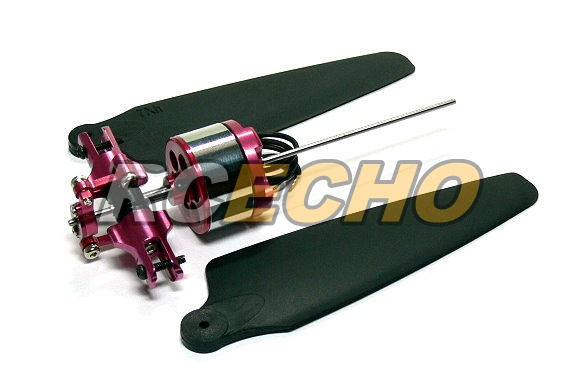
\includegraphics[width = 1\textwidth]{VAPIQ-PICTURES/VPitchAeoc20}
              \caption{AEO C20, Variable Pitch Mechanism}
            \label{fig:vpm}
        \end{minipage}
        \hfill
        \begin{minipage}[b]{0.4\textwidth}
        \centering
            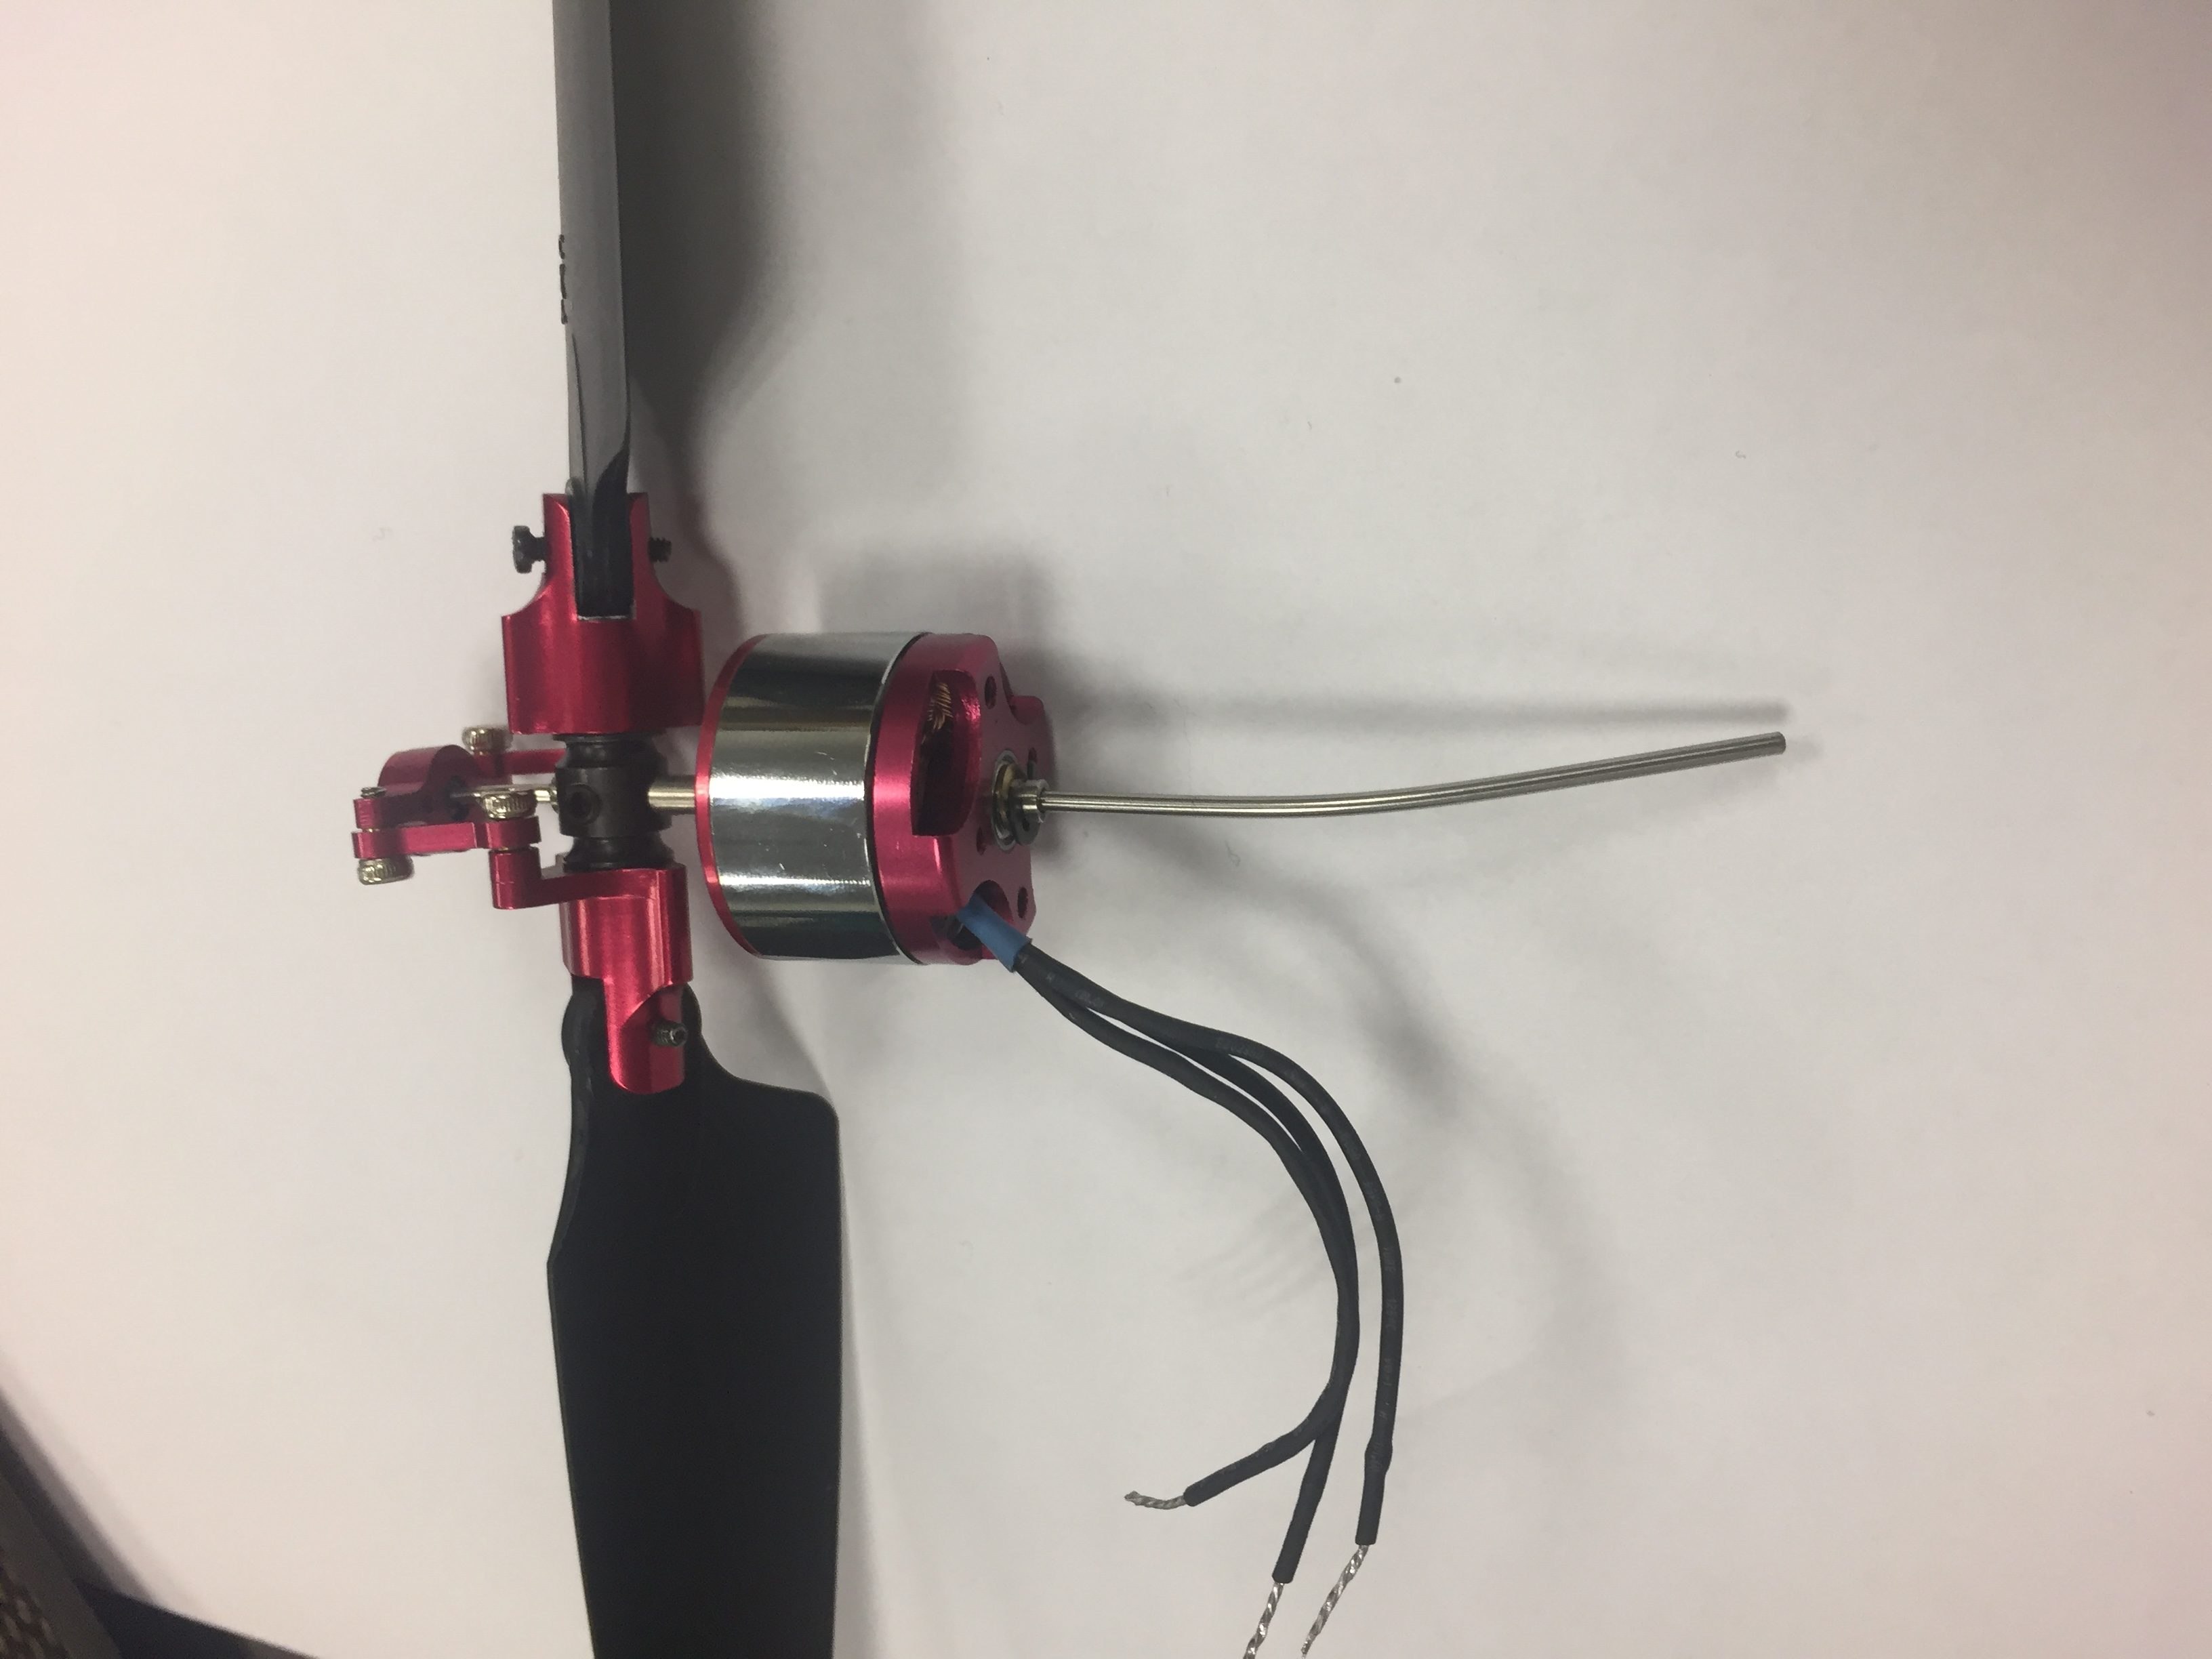
\includegraphics[width = 0.7\textwidth]{VAPIQ-PICTURES/File_004}
            \caption{Recived Item}
            \label{fig:VPQHobbyking}
        \end{minipage}
\end{figure}
\\
The mechanisms was of poor quality, and the shaft on every mechanism was severely bent (Fig. \ref{fig:VPQHobbyking}) and could not be used. By comparing the picture from Hobbyking and the one acquired, we concluded that the mechanism was a fake and not an original part. The team did research on existing variable pitch mechanisms, but there are very few available. This made us consider the tail rotor mechanism of an Align T-rex helicopter. Most RC helicopter-tails have variable pitch, most often with belt drive. If we want to have four separate motors with RPM control, the helicopter tail mechanisms needs to be modified.
\\\\
Additionally in sprint 1, the team got familiar with the motion capture system Qualisys at KIC. To understand the dynamics of a quadcopter, the team also made a simulation Python. (Fig. \ref{fig:simulation}) 

\begin{figure}[h]
        \centering
        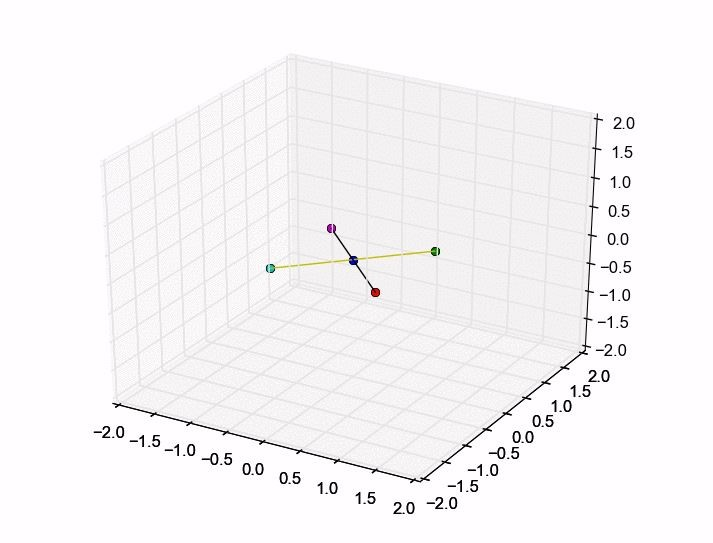
\includegraphics[scale = 0.6]{VAPIQ-PICTURES/simulation}
        \caption{Simulation of Quadcopter Dynamics}
        \label{fig:simulation}
\end{figure}  
\clearpage

\subsection{Completion and Scope Change}

In sprint 1, all activities planned in the project plan were executed and 90 \% of all tasks were accomplished. Some technical tasks was postponed due to documentation and presentation 1. The remaining 10\% of the tasks were reevaluated and brought into sprint 2. There was 5\% scope change, which was due to tasks not identified in the planning phase, concerning documentation. The spike in the graph is due to a change in the way tasks and story points are rated and allocated in JIRA, and is not a real change in scope (Fig. \ref{fig:bds1}). 
\\

\textbf{Projectplan status:}

\begin{figure}[h]
\begin{minipage}[t]{0.5\textwidth}
\textbf{Start-Up Phase:}
\begin{itemize}
	\item Research, \textbf{Done}
	\item Stakeholder Analysis, \textbf{Done}
	\item Documentation, \textbf{Done}
	\item Project Model, \textbf{Done}
	\item Project Plan V.1, \textbf{Done}
	\item Requirements V.1, \textbf{Done}
	\item Test Specification V.1, \textbf{Done}
	\item Document Templates, \textbf{Done}
	\item First Presentation, \textbf{Done}
	\item Presentation 1, \textbf{Done}
    \item Preliminary Documentation Refinement, \textbf{Done}
	\item Presentation Refinement, \textbf{Done}
	\item Presentation Practice, \textbf{Done}
\end{itemize}
\end{minipage}
\hfill
\begin{minipage}[t]{0.5\textwidth}
\textbf{Sprint 1:}
\begin{itemize}
\item Control System Research, \textbf{Done}
    \item Preliminary Flight Simulation, \textbf{Done}
	\item Flight Controller Research, \textbf{Done}
	\item Mechanical Design Study, \textbf{In progress} 
	\item Communication With Qualisys, \textbf{Not completed}
	\item Start Developing Web Page, \textbf{Done}   
\end{itemize}
\end{minipage}
\hfill
\end{figure}\\


Below you can see an extraction of the burndown chart from sprint 1.

\begin{figure}[h]
        \centering
        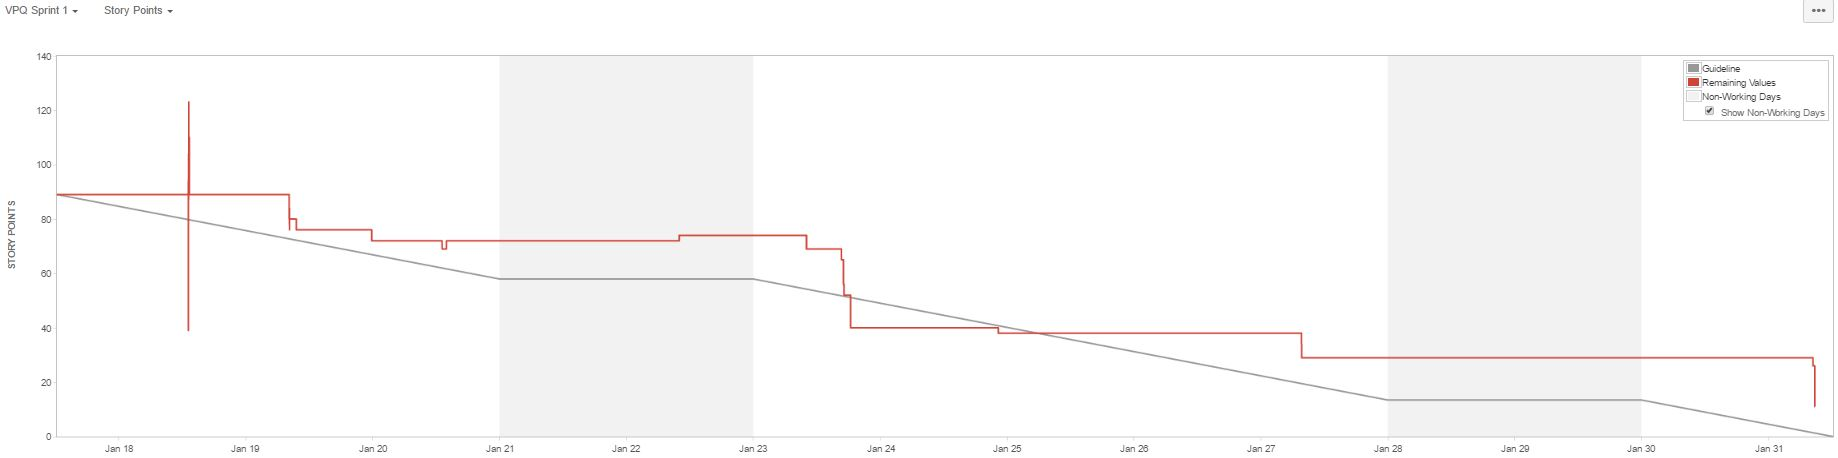
\includegraphics[width = 1\textwidth]{VAPIQ-PICTURES/BDSprint1}
        \caption{Sprint 1 - Burndown Chart}
        \label{fig:bds1}
    \end{figure}  

\subsection{Results and Conclusion}
%Mechanisms did not work, motors was destroyed, could not start the design without the right hardware. Lite penger har utsatt bygging. 

The biggest challenge encountered in Sprint 1 was that the mechanisms we planned to use was of bad quality and we therefore had to reevaluate. Other challenges were time estimation and time-logging. We experienced that estimates of time were often incorrect and we therefore had to make changes on how we planned each sprint.\\

The team got feedback that our motivation for the project was unclear in presentation 1. The team should also minimize the amount of documentation and be more selective of content. Consider making bigger documents instead of many separate. The team also learned to be more sceptical of components from unknown vendors in China.\\
\\
\textbf{The documents produced in sprint 1:}
\begin{itemize}
    \item Organizational Document, containing project
 plan and organization
    \item Backlog And Traceability Document
    \item Test Specification
    \item Qualisys Document
    \item Feasibility Study
    \item Project Model
\end{itemize}
\\\\




